\section{Results}\label{results}
\label{sec:results}
\subsection{Profiling VNTR genotypes across 650 individuals}
\MB{ I want to add following figures to summarize VNTR genotyping in GTEx cohort:}
\begin{enumerate}
    \item Frequency of VNTRs based on their number of alleles (showing that they are mostly non polymorphic and abundance and range of change)
    \item Rate of polymorphism of VNTRs, based on their their annotation (to show we see more variations in non-coding regions)
    \item Distribution of RU count difference compare to reference genome (is it symmetric or we see more expansions compared to deletion). This is not a perfectly symmetric normal distribution.
\end{enumerate}

\subsection{Effect of VNTR variation on gene expression}
\MB{I want to add following figures showing significance of VNTR-eQTLs:}

\begin{enumerate}
    \item Showing gene expression as a function of VNTR genotype for interesting cases
    
    \item Number of unique and shared VNTR-eQTLs for each tissue.
    
    \item A histogram to show how many VNTR-eQTLs are specific to tissue, shared by two tissue, and so on. This is a exponential distribution with most variant as tissue specific (as expected in literature and same as SNVs)
    
    \item A graph comparing VNTRs p-value with SNPs pvalues, showing that most studies miss the the top variant for interesting VNTRs
    
    \item CAVIAR scores for VNTR and nearby SNPS for the interesting VNTRs (causality of VNTR-eQTLs)
    
    \item pairwise correlation of tissues based on pvalue/effect size of their VNTR-eQTLs (and maybe compare it to correlation based on gene expression in those tissues)
    
    \item Effect of distance of the VNTR to the transcription start size on pvalue of the VNTR.
    
    \item for top 10 VNTRs, show the tissues that they are affecting and their significance
\end{enumerate}

\subsection{Neural Recruitment Results}
To we present the result of our experiments, first we describe the baseline methods that we chose for our comparisons. Then, we proceed by describing our efforts for tailoring our model and improve the method. Finally, we provide a comprehensive analysis of the performance of our method and the comparison with the baselines.

\paragraph{Comparison with fast alignment methods.}
The current gold standard for finding the location of reads in the genome are alignment tools \cite{Langmead2012}. These methods are mainly designed to analyze sequencing reads in an efficient way and identify their location. While they work perfectly accurate in most situations, they will fail for the cases with a significant change in the genome of the sample and subsequently in the reads. We use Bowtie 2 as our first baseline which is designed to be fast and practical, but has lower sensitivity compare to specialized methods of second baseline.

\paragraph{Comparison sensitive graph based models.}
To overcome the limitation of common alignment tools, several efforts have been made by discounting running time. In particular, representing genome with graph instead of a static sequence is known to increase the sensitivity of alignment for targeted cases \cite{Rakocevic2019}. This approach is also being used in identifying the variations in tandem repeats of the human genome \cite{Bakhtiari2018, Dolzhenko2019}. Of these two implementation, one is aligning sequencing reads to graphs made by strings and another is building the graph using Hidden Markov Model to obtain higher sensitivity and allowing variations within repeating units. We use the HMM implementation in adVNTR package to have highest read identification recall for the second baseline.

\paragraph{Choosing the optimal k-mer length}
The choice off k-mer length depends on the application. For example, increasing the k-mer size could decrease sensitivity in our case as a small variation will significantly change the k-mer composition, whereas lowering k-mer size reduces the features that are identifier of a pattern \cite{Zhang2017}. In addition, our embedding size exponentially grows with respect to the $k$ so there is also a practical upper bound on the $k$. Following Zhang \yrcite{Zhang2017} and Dubinkina \yrcite{Dubinkina2016}, we trained and tested in the range $4\le k<9$. The accuracy remains comparable in this range (Fig.~\ref{fig:kmer_length}), and we chose $k=6$ as its mean validation accuracy is the highest compare to four other values of $k$.
\begin{figure}[ht]
\vskip -0.11in
\begin{center}
\centerline{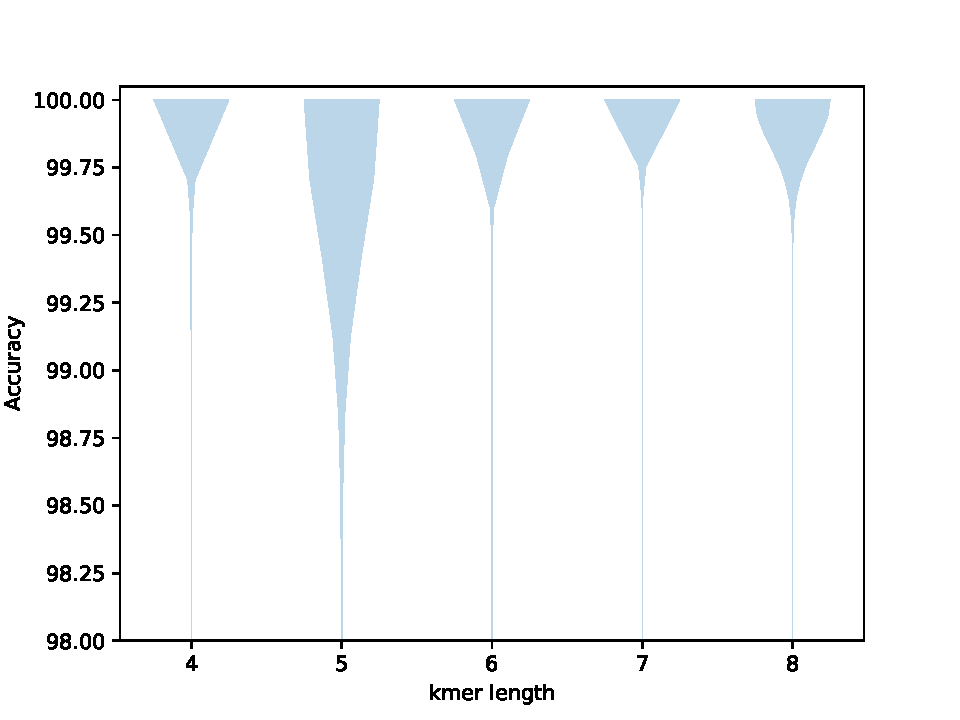
\includegraphics[width=\columnwidth]{fig/kmer_length.pdf}}
\caption{\footnotesize{\bf Effect of kmer length on accuracy.}
 Performance of our model on validation set for different k-mer lengths.}
  \label{fig:kmer_length}
\end{center}
\vspace{-0.3in}
\end{figure}

\paragraph{Effect of different loss functions}
To explore how choosing a loss function improves the performance of our model, we obtained the validation performance of our model for three binary classification loss functions (Cross-entropy, Hinge, Squared Hinge) and three regression loss functions (MSE, MAE, and MSLE). Each distribution in Fig. ~\ref{fig:loss_function} shows the accuracy of a loss function on validation set across 1905 genomic loci. We analyzed these distributions using one-way analysis of variance (ANOVA) and none of them were significantly better than others. Therefore, we chose Cross-entropy since it has the highest mean accuracy (99.95\%) among loss functions and its binary classification nature fits our problem.
\begin{figure}[!ht]
\vskip -0.11in
\begin{center}
\centerline{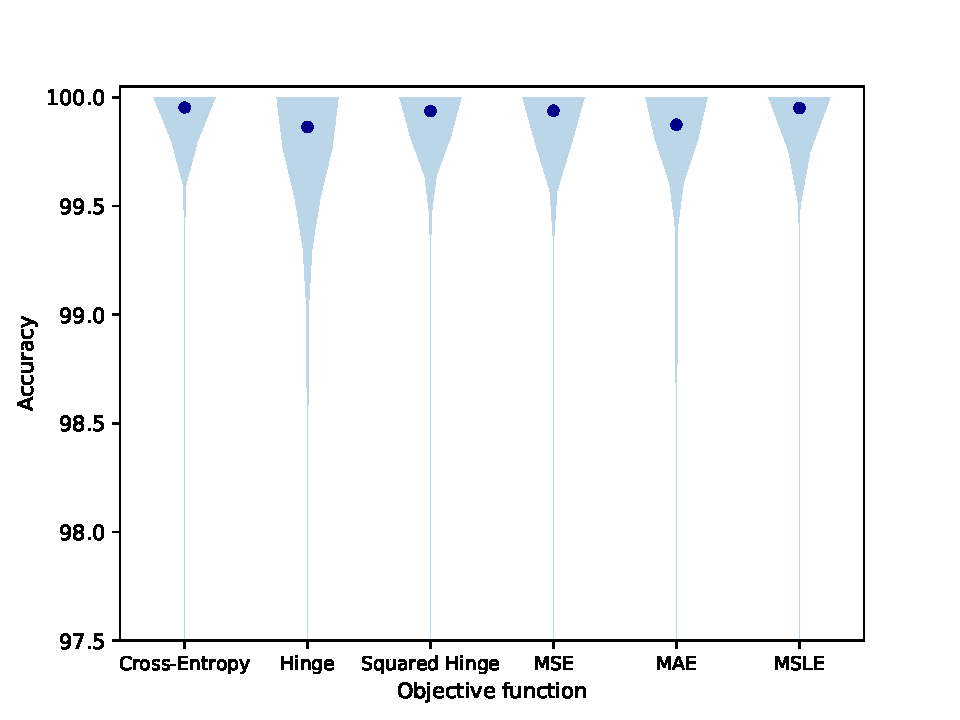
\includegraphics[width=\columnwidth]{fig/loss_function.pdf}}
\caption{\footnotesize{\bf Effect of loss function on accuracy.}
 Performance of our model on validation set for different loss functions. The mean of each distribution is shown by a blue dot.}
  \label{fig:loss_function}
\end{center}
\vspace{-0.3in}
\end{figure}

\paragraph{Qualitative analysis}
To assess the quality of our method, we compare it with two baselines. As the data are very imbalanced we use both precision ($\frac{TP}{TP+FP}$) and recall ($\frac{TP}{TP+FN}$) to assess the selection quality, instead of a single accuracy value\cite{Zou2018}. Fig.\ref{fig:accuracy} shows a scatter plot of the precision and recall of read selection for each VNTR locus using three methods. Using neural network, 99\% of the loci have at least 95\% recall, while only 6\% and 91\% of the loci have these recall using Bowtie 2 and HMM, respectively. In terms of precision, all three methods have full precision for at least 96\% of all loci and Bowtie 2 and our method achieve the highest precision for the remaining loci.
\begin{figure}[ht]
\vskip -0.1in
\begin{center}
\centerline{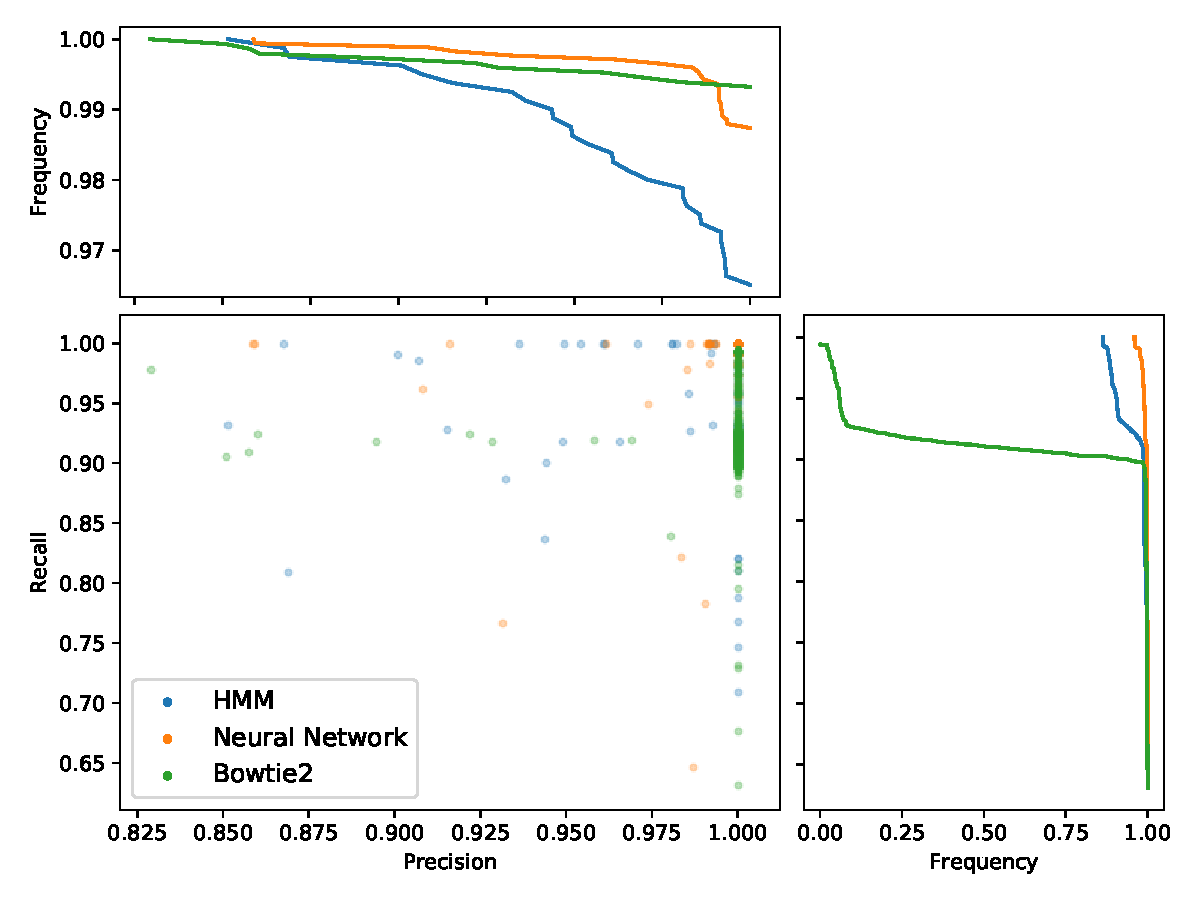
\includegraphics[width=\columnwidth]{fig/accuracy.pdf}}
\caption{\footnotesize{\bf Accuracy of VNTR genotyping.}
 The scatter plot shows precision and recall of classification with different methods. Each point represent a VNTR locus. So, there are total of 1905 points for each color/method. Also, cumulative distributions of precisions and recalls on the sides show most of the points have high precision and recall using neural network.}
  \label{fig:accuracy}
\end{center}
\vspace{-0.3in}
\end{figure}

\paragraph{Classification speed}
The distribution of running time of each test data for three methods is shown in Fig. \ref{fig:running_time}. Our method has a mean of 1.1 seconds and 25th percentile of 0.3 seconds to do the classification for each locus. The baselines have mean of 4.4 and 204.7, and 25th percentile of 3.1 and 23.6 seconds, respectively, to classify the reads for each locus.
\begin{figure}[ht]
\vskip -0.1in
\begin{center}
\centerline{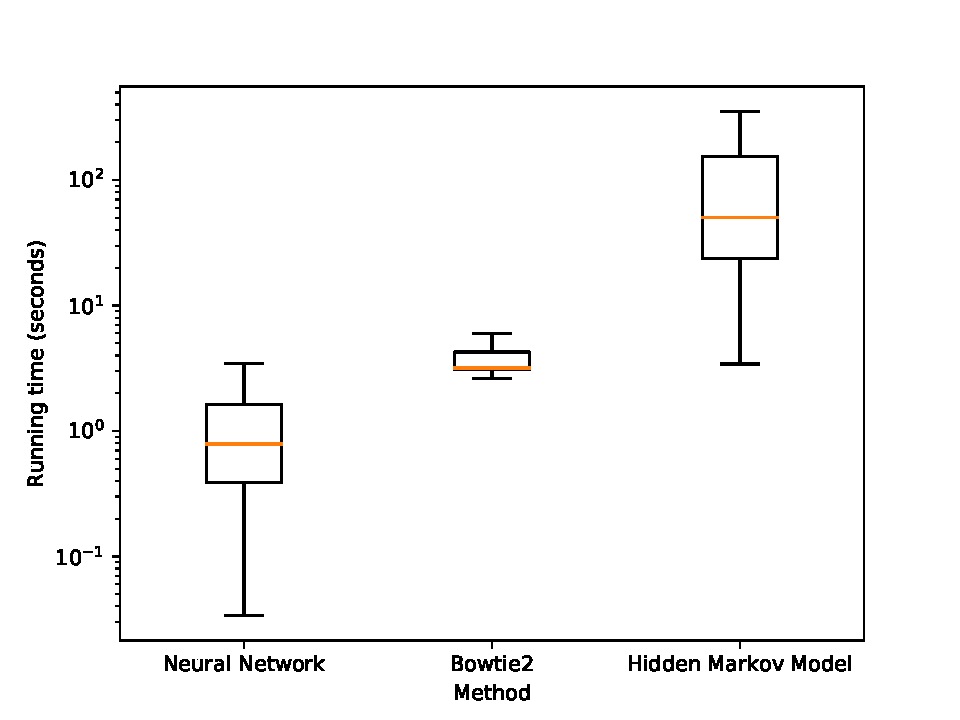
\includegraphics[width=\columnwidth]{fig/hmm_dnn_running_time.pdf}}
\caption{\footnotesize{\bf Running time of read classification.}
 Each box shows the distribution of running time per locus for one method. As expected, second baseline that is sensitive method has the highest average running time.}
  \label{fig:running_time}
\end{center}
\vspace{-0.3in}
\end{figure}

